\section{What Determines Distillability?}\label{sec:distillability}

\subsection{Teacher-state reversal at fixed composition}
\label{sec:teacher-state}
At the same $\alpha=0.5$, jointly trained J has teacher validation-subset NLL 4.300644, compared with 6.376220 for fusion-weight-only A. J improves all three students by $+0.155665\pm0.007692$ NLL, whereas A harms all three with gain $-0.027654\pm0.006822$. The paired state contrast is
\begin{equation}
Q=\mathrm{NLL}_{\mathrm{KD,A}}-\mathrm{NLL}_{\mathrm{KD,J}},
\label{eq:teacher-state-contrast}
\end{equation}
averaging $+0.183319\pm0.001375$, positive in all three seeds.

Teacher training state and resulting predictive quality strongly modulate transfer at fixed architecture and composition. This is not scalar-likelihood causality: joint training also changes representations and errors, and teacher training budgets differ. Appendix~\ref{app:protocols} retains the original modes and eligibility amendments.

\subsection{A weaker source still transfers positively}
\label{sec:weaker-teacher}
The Grassmann-only source has validation-subset NLL 4.652064, worse than every matched validation-selected CE comparator on that subset. Nevertheless, all three students improve, with mean test gain $+0.040991\pm0.006733$. The comparator is the selected CE continuation, not an arbitrary initialization. Teacher likelihood is compared against the matched CE endpoint on the same validation subset, whereas transfer gain is evaluated on the selected test endpoints (Appendix~\ref{app:per-seed}).

Together, these controls show that teacher quality matters strongly but global held-out likelihood alone is insufficient to determine useful supervision. They neither make teacher quality irrelevant nor attribute positive transfer to geometry (Figure~\ref{fig:teacher_quality}).

\begin{figure*}[!t]
\centering
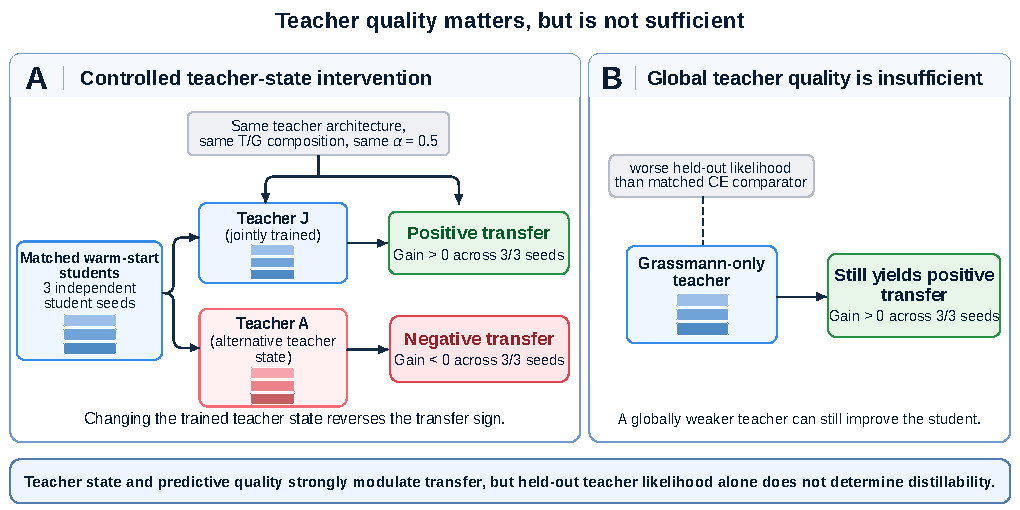
\includegraphics[width=\textwidth]{figures/fig3_teacher_quality.pdf}
\caption{WikiText-2 state and likelihood controls. Changing trained teacher state reverses transfer at fixed composition; a source with worse likelihood than CE still transfers positively. Neither establishes scalar-likelihood causality or a geometric KD advantage.}
\label{fig:teacher_quality}
\end{figure*}
